\documentclass[11pt]{article}

% ---------- packages ----------
\usepackage[margin=1in]{geometry}
\usepackage{amsmath,amssymb}
\usepackage{graphicx}
\usepackage{xcolor}
\usepackage{booktabs}
\usepackage{microtype}
\usepackage{caption}
\usepackage[hidelinks]{hyperref}
\usepackage{enumitem}
\usepackage[numbers,square]{natbib}

% ---------- authoring tags (visible, NOT part of final prose) ----------
% These mirror the outline's tags so unverified material never hides as fact.
\newcommand{\VERIFY}[1]{{\color{red}\small\textsf{[VERIFY: #1]}}}
\newcommand{\CHECK}[1]{{\color{orange!80!black}\small\textsf{[CHECK: #1]}}}
\newcommand{\NEXTPAPER}[1]{{\color{gray}\small\textsf{[NEXT-PAPER: #1]}}}
\newcommand{\todofig}[2]{%
  \begin{figure}[t]\centering
  \fbox{\parbox[c][3.2cm][c]{0.86\linewidth}{\centering
  {\color{red}\textsf{[FIGURE TO GENERATE]}}\\[4pt]
  \small #1}}
  \caption{#2}
  \end{figure}}

\title{\bfseries Faithful per-layer geometric readout of the ESMFold trunk,\\
and the energy-manifold adherence it reveals}
\author{William Klett\\\small Princeton University}
\date{Draft --- \today}

\begin{document}
\maketitle

% =====================================================================
\begin{abstract}
\noindent
We introduce a \emph{faithful per-layer geometric readout} of the ESMFold trunk:
a distogram autoencoder trained, at each block, to reconstruct that block's pair
representation $z_t$, and minimize KL divergence between the next block, ultamitely 
encouraging physicality in the distogram readout. We find this method succesfull
at receovering the protein folding dynamics of the trunk's intermediate layers, maintaning plausible, 
euclidian readouts without any direct geometric supervision. 
Using it, we find that the trunk's intermediate geometric beliefs trace a path that adheres to the
energy manifold: the model folds the protein into its final state through a trajectory 
that monotonically decreases energy between each succesive layer. The consistency of this 
finding striking---even proteins that end up in a locally non-optimal conformation still follow an 
energy-decreasing path, indicating that energy itself may be partially determining the path of folding trajectories.
To our knowledge, this is first faithful investigation into the dynamics of geometric 
representations within a single-pass protein structure predictor.
\end{abstract}

% =====================================================================
\section{Introduction}
\label{sec:intro}

\paragraph{The gap.}
Single-pass structure predictors such as ESMFold are accurate but mechanistically
opaque. The trunk iteratively refines a pair representation
$z \in \mathbb{R}^{L\times L\times 128}$ over $\sim$48 blocks
\CHECK{confirm exact block count for the cached model (47/48)} and emits a single
prediction with no recycling and no MSA. Reading the trunk's \emph{intermediate}
states faithfully would show \emph{how} a structure assembles, not merely
\emph{that} it does.

\paragraph{Two questions, one of them open.}
Interpretability of these models divides into two questions: \emph{what the model
is thinking about}---the content that is decodable from a representation (linear
probes, sparse autoencoders)---and \emph{what those thoughts are}---the model's
own evolving belief. The first is well studied; the second is not, because the
obvious instruments for it are confounded (\S\ref{sec:prior}). This paper answers
the second, faithfully, for the trunk's geometric belief.

\paragraph{Contributions.}
\begin{enumerate}[leftmargin=1.3em,itemsep=2pt]
\item \textbf{A faithful per-layer geometric readout.} A distogram autoencoder
  probe per block, trained on reconstruction of $z_t$ plus adjacent-layer
  consistency, anchored only at the in-distribution final layer to the model's
  own head---no native structure in the loss
  (\S\ref{sec:faithful},\,\S\ref{sec:probe-construction}). We give the
  faithfulness criterion it is built on and validate it
  (\S\ref{sec:faithful-validation}).
  \NEXTPAPER{resolve the readout's name vs.\ the prior ``PSA'' (physical
  structure autoencoder) paper to avoid collision.}
\item \textbf{The finding it enables.} The trunk's intermediate beliefs trace a
  trajectory that adheres to the low-energy manifold even on incorrect folds,
  while a direct path between the same endpoints tunnels through forbidden
  high-energy geometry (\S\ref{sec:finding}). 
\end{enumerate}

\paragraph{Roadmap.}
Section~\ref{sec:prior} situates the method against prior interpretability work
and derives the faithfulness criterion. Section~\ref{sec:finding} presents the
energy-manifold results. Sections~\ref{sec:limitations}--\ref{sec:conclusion}
give bounds, directions, and a closing synthesis.

% =====================================================================
\section{Prior work and what faithfulness requires}
\label{sec:prior}

\subsection{Two kinds of interpretability question}
\label{sec:two-questions}

\emph{What the model is thinking about} (decodable content). Linear probes and
sparse autoencoders treat the representation as something to extract from---an
external instrument measuring what is recoverable.
\begin{itemize}[leftmargin=1.3em,itemsep=1pt]
\item Sparse autoencoders: InterPLM \citep{simon_interplm};
  \citet{adams_sae}; the Reticular Matryoshka-SAE on ESM2-3B
  \citep{reticular_msae}. \VERIFY{each does what is attributed; read methods, not
  abstracts.}
\item Linear decoders: \citet{lu2026phase} (phase diagram of distance
  decodability by depth); AlphaInterp on AlphaFold~3 \citep{alphainterp}.
  \VERIFY{attribution.}
\end{itemize}

\emph{What those thoughts are} (the model's evolving belief). The natural move is
to apply the model's own output interface to an intermediate state---but this has
two problems.

\subsection{The second camp's two problems}
\label{sec:two-problems}

\paragraph{Problem 1: the distogram head is out of distribution on intermediate
layers.}
ESMFold's distogram head is trained on the distribution of \emph{final-layer}
representations. Applied mid-trunk it is out of distribution, and it shows it:
the implied distance maps violate the triangle inequality across a wide middle
band of layers (the ``M-curve,'' Fig.~\ref{fig:violation-curve}). This is a
contradiction in the field's joint commitments: geometry is reported to be
\emph{linearly decodable} from $z$ into Euclidean space \citep{lu2026phase}
\VERIFY{that linear-decodability is attributable to Lu et al.}, yet the head's
intermediate readout is \emph{non-metric}. Both cannot describe the same
representation. The resolution: the non-metricity belongs to the
\emph{instrument}, not to $z$.

\paragraph{Problem 2: ground-truth-supervised per-block readouts measure the
wrong thing.}
AlphaFold retrains a structure module per block against native structure
\citep{alphafold2} \VERIFY{native-supervised per-block readout, Supp.\ Methods
1.14}. This avoids the OOD problem but measures \emph{downstream sufficiency},
not \emph{content}: how recoverable the final answer is from layer $t$, not what
layer $t$ represents.

\emph{The proof analogy.} One could train a model to complete a proof from any
single line; its success rate measures how \emph{determined} the conclusion is by
that line, not what the line \emph{says}. A native-supervised per-block readout
reads the proof's completability, not the content of the line. The consequence
matters here: a confidently \emph{wrong} intermediate belief has definite
content---a specific wrong geometry---but a ground-truth decoder can only report
low decodability and will miss that a coherent wrong belief is present. (This is
exactly the regime our false-fold results in \S\ref{sec:false-protein} probe.)

\subsection{What faithfulness requires}
\label{sec:faithful}

We define the trunk's geometric belief at layer $t$ as the distance distribution
that, among all distance distributions, best \emph{reconstructs} $z_t$.
\begin{itemize}[leftmargin=1.3em,itemsep=1pt]
\item \textbf{Reconstruction fidelity to $z_t$, not predictive fidelity to
  native.} Reading content, not implication.
\item \textbf{Restriction to distance distributions.} Reading the \emph{geometric}
  belief specifically, projecting out sequence/coevolutionary content.
\end{itemize}
Reconstruction is the right content criterion for a causal reason: $z_t$ is what
the downstream trunk actually consumes, so reconstruction-recoverable content is
exactly the content that flows forward. The probe reads what the network reads; a
native decoder reads what an external instrument can extract, which need not
coincide.

\subsection{Probe construction}
\label{sec:probe-construction}

At each block $t$ we train a per-pair bottleneck,
\texttt{PairDistogramBottleneck} (\texttt{pair\_dim}$=128$, \texttt{bins}$=64$,
\texttt{hidden\_dim}$=256$), that maps a single pair vector $z_t[i,j]$ to a
64-bin distogram over the same distance grid ESMFold's own head uses
($\approx 2.3$--$21.7$\,\AA), then decodes back to $z_t[i,j]$. The loss has
exactly two per-pair terms:
\begin{equation}
\mathcal{L}_t \;=\;
\underbrace{\big\| \,\mathrm{dec}(\mathrm{enc}(z_t[i,j])) - z_t[i,j]\,\big\|^2}_{\text{reconstruction of } z_t}
\;+\;
\lambda\,\underbrace{\mathrm{KL}\!\big(\mathrm{enc}(z_t[i,j]) \,\big\|\, p^{\text{tgt}}_t[i,j]\big)}_{\text{adjacent-layer consistency}} .
\end{equation}

\paragraph{Linking-back anchoring.}
The layer-46 probe's consistency target $p^{\text{tgt}}_{46}$ is ESMFold's own
distogram head applied to $z_{47}$---the head used \emph{in distribution}, at the
layer it was trained for. Each earlier probe is anchored to the just-trained next
probe: $p^{\text{tgt}}_t = \mathrm{enc}_{t+1}(z_{t+1})$. The chain is anchored
only at the final, in-distribution layer; no native structure enters at any
point.

\paragraph{Iterative-refinement assumption (imported).}
Reading distances block by block presupposes that geometric content changes
\emph{gradually} across blocks, so each backward link is a small extrapolation
from a good anchor. We state this as an assumption, supported by prior evidence
that distance/geometric content accumulates progressively through the trunk
\citep{lu2026phase} \VERIFY{phase-diagram / gradual-accumulation attribution}; we
do not prove it here.

\subsection{Faithfulness validation: the changes are geometric}
\label{sec:faithful-validation}

\paragraph{The core argument.}
Reconstruction forces each probe to encode whatever distinguishes its layer. That
information is either geometric or non-geometric---two cases with opposite
signatures.
\begin{description}[leftmargin=1.4em,itemsep=2pt]
\item[Case 1 (non-geometric).] Forcing layer-distinguishing information through a
  per-pair \emph{distance} code mis-encodes it. Because probes are chained, the
  Euclidean fraction would decay multiplicatively with distance from the anchor:
  embedding stress would rise monotonically toward early layers and triangle
  violations would accumulate.
\item[Case 2 (geometric).] Independent per-pair readouts come out mutually
  metric-consistent with \emph{no} enforcement: stress stays flat and low, and
  violations stay at zero at all depths.
\end{description}

\paragraph{We observe Case 2.}
Across 57 proteins (good and bad folds) and all 46 layers, sampling random
triples $(i,j,k)$ and checking $d(i,k) > d(i,j)+d(j,k)$, the violation rate is
$0.0000$ ($\sim$8M triple-checks).
\CHECK{re-confirm the exact triple count and that the rate is identically zero at
every depth, not just on average.}
Embedding stress is flat across depth and low---comparable to the embedding error
of the native structures themselves ($\sim$5--12\,\AA, Fig.~\ref{fig:stress})---
even for the protein whose final TM-score is near zero.
\CHECK{report the stress band precisely and the per-layer reconstruction $R^2$;
confirm no early-layer reconstruction degradation.}

\paragraph{The clincher.}
Nothing in the loss enforces Euclidean structure: no cross-pair coupling, no
embedding term. The probe is \emph{free} to be non-metric---and the model's own
head, with the identical freedom, \emph{is} non-metric on the same layers
(Fig.~\ref{fig:violation-curve}). The probe is not. Unforced metric-consistency
of independent per-pair readouts is possible only if $z$ encodes coherent
geometry for them to read. This is the methodological centerpiece: the contrast
between the head's M-shaped violation curve and the probe's flat-zero curve.

\todofig{Paired triangle-inequality violation rate across trunk depth:
ESMFold's own head applied to intermediate $z_t$ (M-shaped, violations across the
middle band) vs.\ the faithful probe (flat at zero, all depths). Generate with
\texttt{scripts/eval\_triangle\_violations.py} extended to also evaluate the
native head per layer; \texttt{scripts/plot\_triangle\_inequality.py} for the
figure.}
{Methodological centerpiece. The head is non-metric mid-trunk; the probe, with
the same freedom, is metric-consistent at every depth---so the geometry is a
property of $z$, read faithfully by the probe, not an artifact of the readout.
\label{fig:violation-curve}}

\begin{figure}[t]\centering
  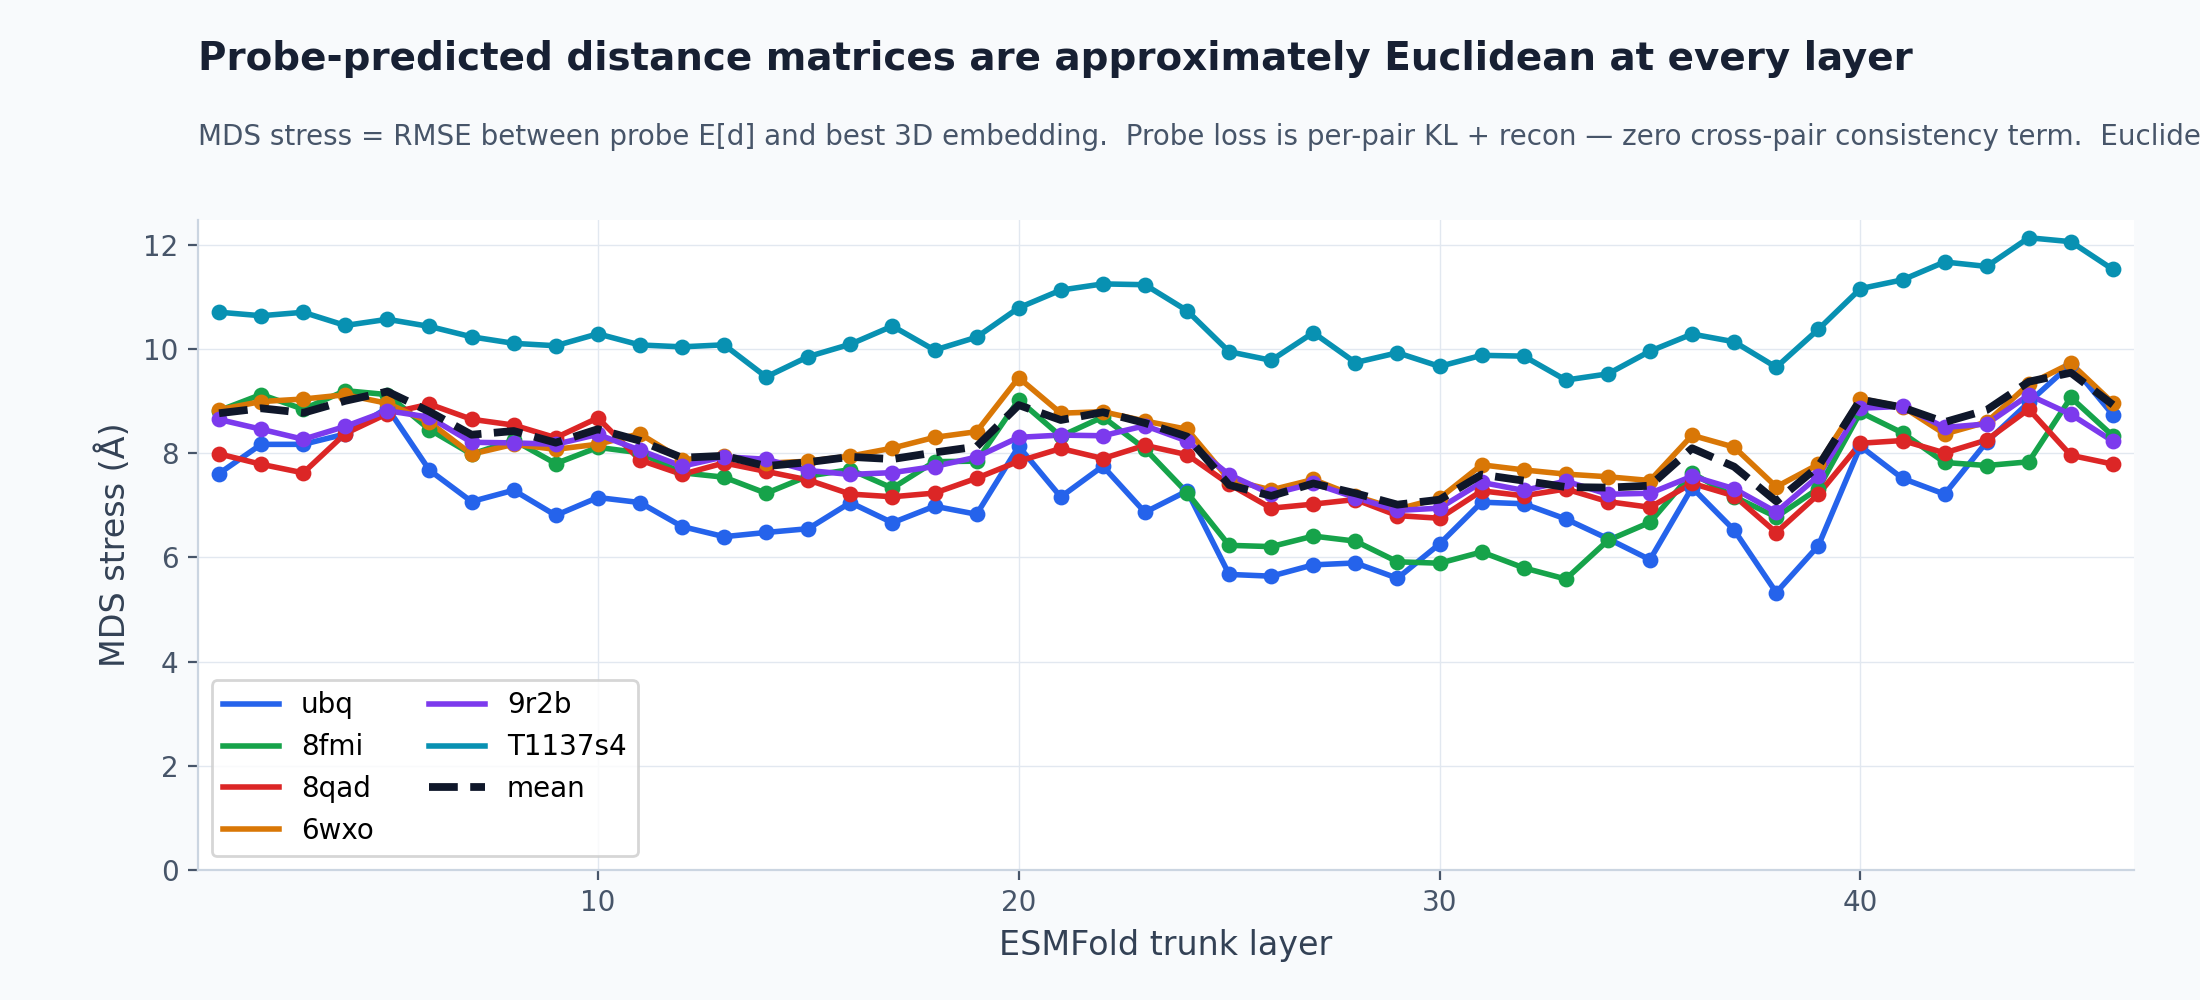
\includegraphics[width=0.78\linewidth]{figures/stress_by_layer.png}
  \caption{MDS embedding stress of the probe-read distance matrix across all 46
  trunk layers, for six benchmark proteins. Stress is flat and low at every
  depth---no growth toward early layers---consistent with Case 2: the probe reads
  coherent geometry rather than mis-encoding non-geometric content.
  \CHECK{add the native-structure embedding-error reference line.}}
  \label{fig:stress}
\end{figure}

% =====================================================================
\section{The trunk's beliefs adhere to the low-energy manifold}
\label{sec:finding}

\noindent\textbf{Topic sentence.} The trunk's intermediate structures trace a
trajectory that adheres to the low-energy manifold, even when the model folds
incorrectly.

\subsection{The observation that prompted the question (motivation, not evidence)}
\label{sec:animation}

Watching the MDS-embedded intermediate structures evolve (fixed camera,
Kabsch-aligned to the final layer), the trunk makes large, \emph{coherent} global
reconfigurations---and does so even on proteins it ultimately folds incorrectly.
Two things are apparent: the moves are large, and the moves are clean
(coordinated, not thrashing). The puzzle: a large reconfiguration generically
passes through bad geometry (clashes, high energy), yet the trunk's moves appear
not to. Does the trajectory respect the energy landscape even during large moves,
even when folding wrong? We frame this as motivation; the quantitative tests
follow. The claim is ``large coherent moves even when wrong,'' not ``wrong folds
move more''---the latter is unneeded.

\begin{figure}[t]\centering
  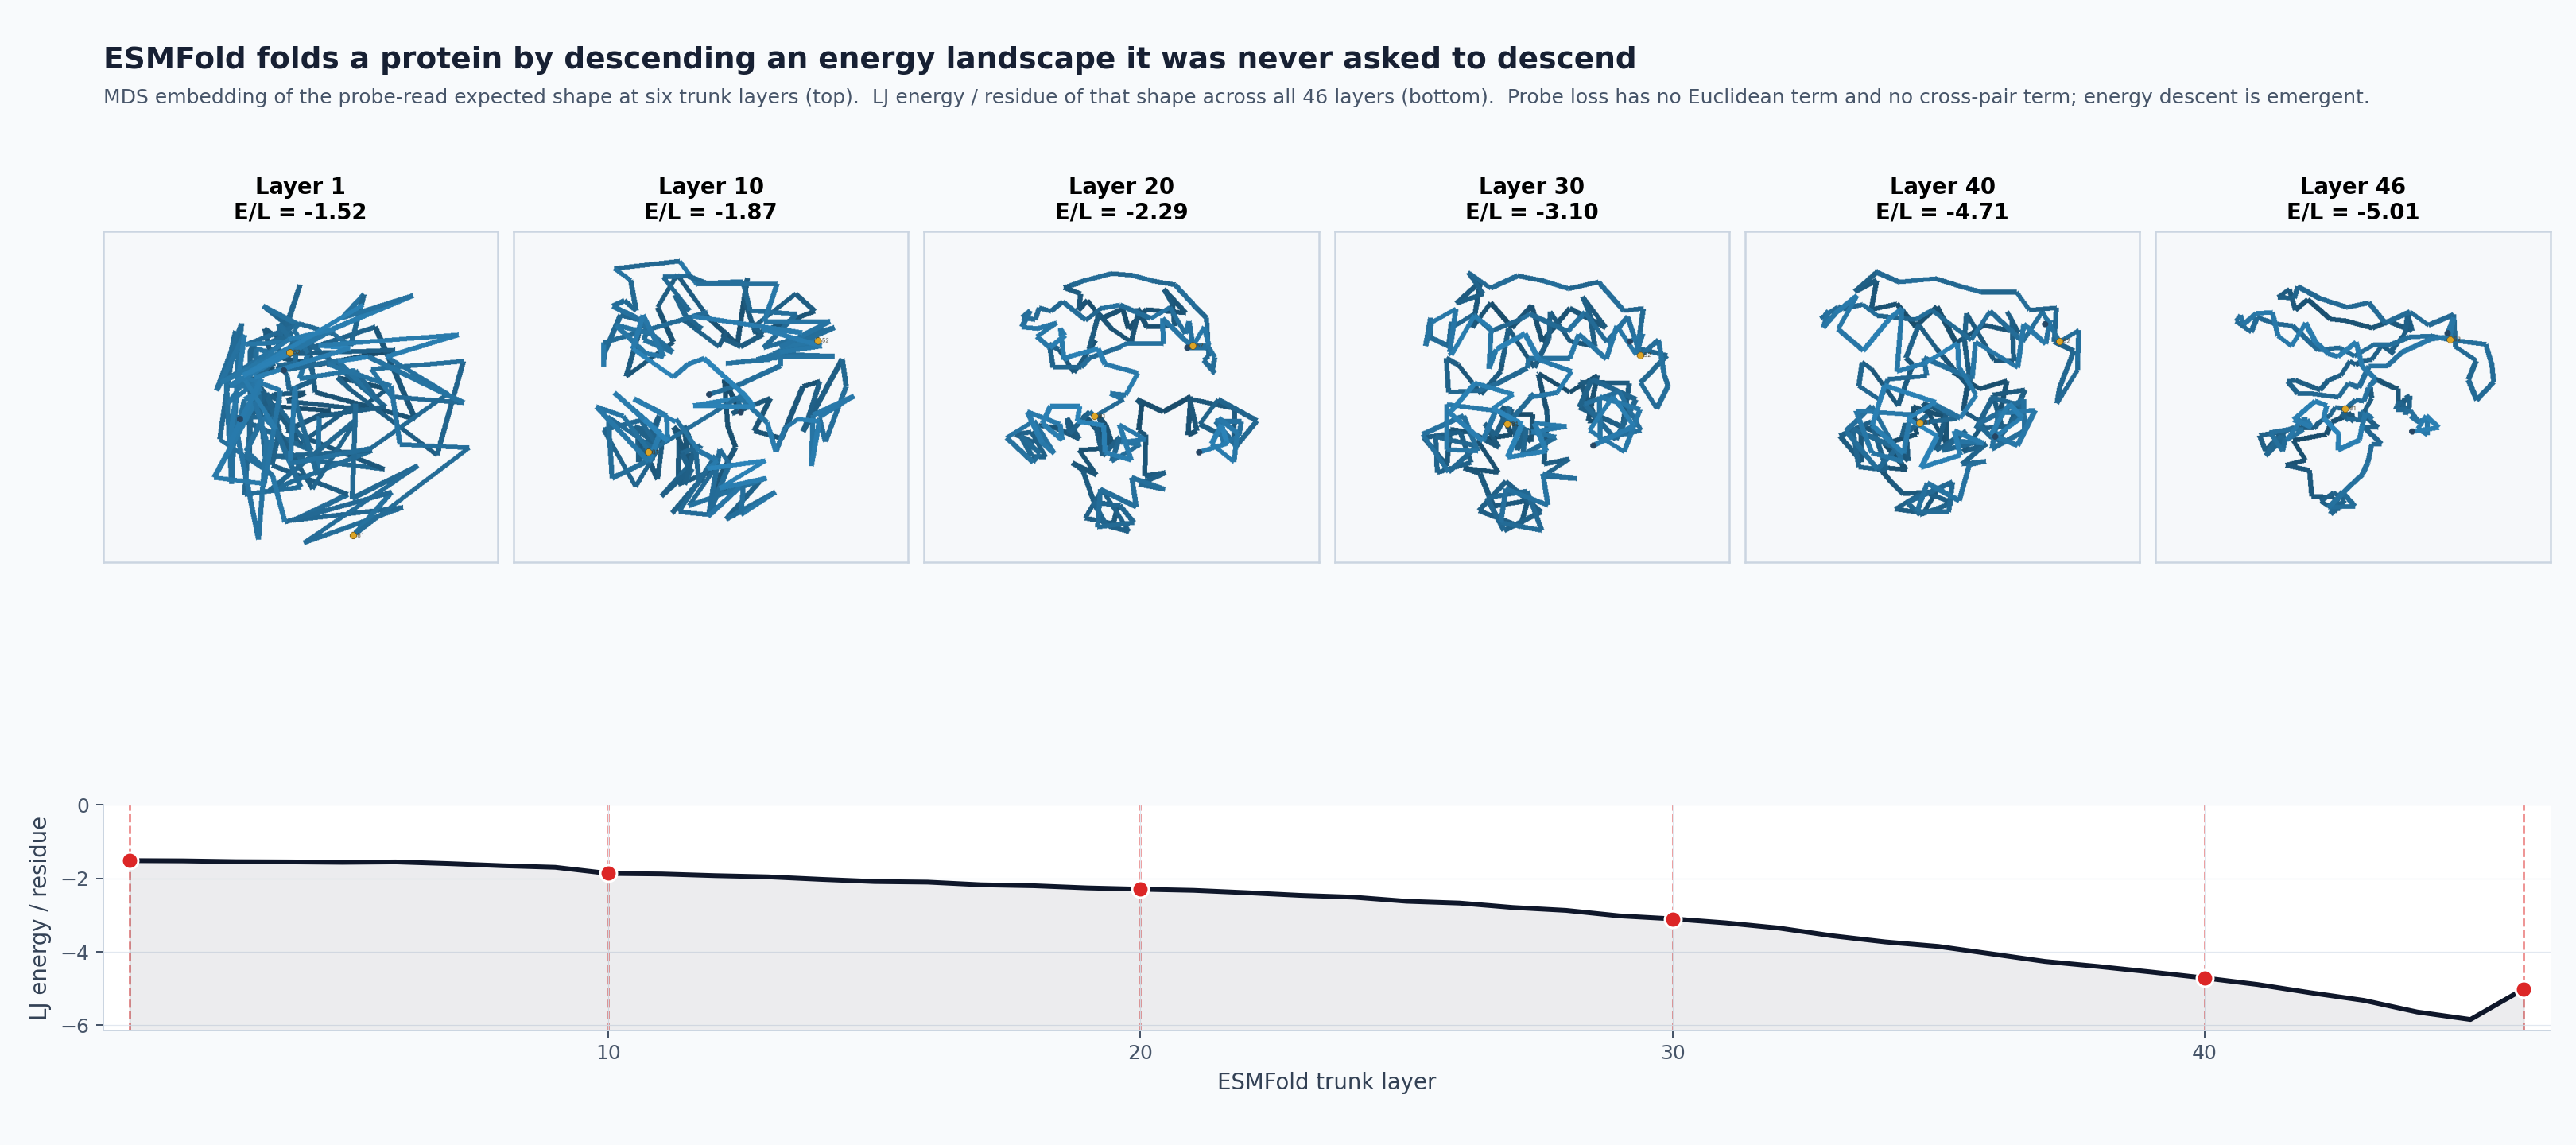
\includegraphics[width=0.95\linewidth]{figures/keyframe_energy.png}
  \caption{Keyframe montage of one protein's probe-read intermediate structures
  (fixed camera, aligned), with the per-layer energy curve beneath. The structure
  self-assembles through large, coordinated motions; the energy descends in
  lockstep. Motivation for the quantitative tests in
  \S\ref{sec:descent}--\S\ref{sec:not-gd}.}
  \label{fig:keyframe}
\end{figure}

\subsection{Energy descends along the path---and the descent is packing, not
clash-avoidance}
\label{sec:descent}

We compute the Lennard-Jones energy of the probe's expected shape per layer,
\begin{equation}
E_t \;=\; \frac{1}{L}\sum_{|i-j|>3} 4\varepsilon\!\left[
\left(\tfrac{\sigma}{\mathbb{E}[d_t(i,j)]}\right)^{12}
-\left(\tfrac{\sigma}{\mathbb{E}[d_t(i,j)]}\right)^{6}\right],
\qquad \sigma=6.8\,\text{\AA},\ \varepsilon=1,
\end{equation}
and observe a near-universal monotone decrease through the trunk
(Fig.~\ref{fig:energy-grid}).

\paragraph{Two distinct energy phenomena, kept separate.}
\begin{enumerate}[leftmargin=1.4em,itemsep=2pt]
\item[(i)] \emph{Path-level steric adherence} (\S\ref{sec:chord}): the trunk's
  \emph{route} stays in the non-overlapping region; driven by the repulsive
  $r^{-12}$ wall; dramatic magnitude (clashes $\to 10^3{+}$); a geometric /
  excluded-volume claim.
\item[(ii)] \emph{Within-manifold packing descent} (this subsection and
  \S\ref{sec:not-convergence}--\S\ref{sec:false-protein}): among already-valid,
  clash-free configurations, the trunk moves toward more favorably-packed ones;
  driven by the attractive/soft part of the potential; modest magnitude.
\end{enumerate}
These do different jobs (boundary adherence vs.\ interior optimization); neither
reduces to the other.

\paragraph{The descent is not the repulsive term---an argument from magnitude.}
The monotone decrease through the trunk is of order $\sim$5--10 per residue.
Steric clashes under the \emph{same} potential produce changes of order $10^3$
and above (the chord spike, \S\ref{sec:chord}), because $r^{-12}$ blows up on
overlap. The repulsive wall is effectively a step---clashing ($10^3{+}$) or not
($\approx 0$)---with no regime that contributes a smooth change of size 5--10.
Therefore a smooth descent of order 5--10 is far too small to be escape from the
repulsive wall; it must reflect refinement in the soft, attractive, clash-free
regime: the trunk improving favorable packing among configurations that are
already physically valid. A second angle gives the same conclusion: the minimum
interatomic distance stays comfortably above contact distance \emph{throughout}
the descent phase---there is no clash to escape while energy is descending.
\CHECK{report min-interatomic-distance during the descent phase; available from
the \S\ref{sec:chord} analysis.}

\begin{figure}[t]\centering
  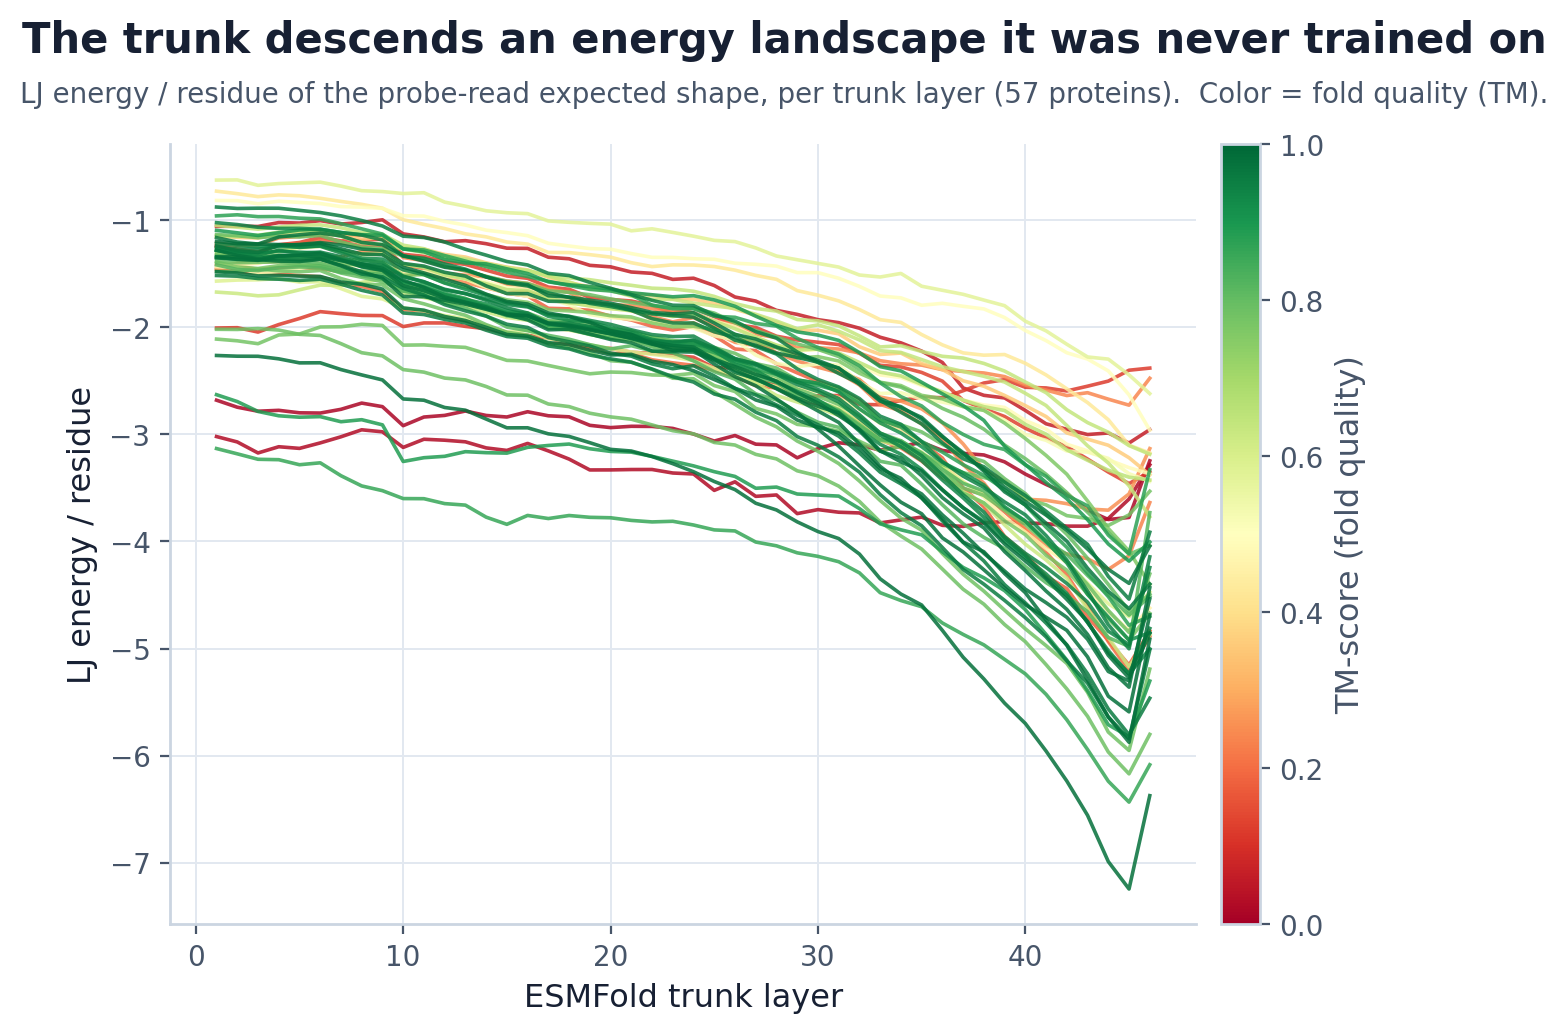
\includegraphics[width=0.95\linewidth]{figures/lj_energy_grid.png}
  \caption{Per-protein LJ energy of the probe's expected shape across the trunk,
  arranged by fold quality. Descent is near-universal; deeper, smoother descents
  belong to better folds. The decrease is of order 5--10/residue---far below the
  $10^3{+}$ scale of steric clashes (\S\ref{sec:chord})---so it reflects packing
  refinement within the clash-free regime, not escape from overlap.}
  \label{fig:energy-grid}
\end{figure}

\noindent Why it matters: a model that merely avoided clashes would be
unremarkable; a model that smoothly, monotonically improves packing favorability
\emph{among valid structures}---even on wrong folds
(\S\ref{sec:false-protein})---is doing something optimization-like. The magnitude
argument licenses calling the descent optimization rather than triviality. The
immediate deflation to rule out next: is this just convergence toward the (low-energy)
answer?

\subsection{The packing descent is not just convergence (within-protein)}
\label{sec:not-convergence}

\emph{Deflation.} Is the packing descent merely convergence toward the
low-energy answer? A byproduct reading predicts that the rate of geometric
approach to the destination and the rate of energy descent are positively coupled.

\emph{Result.} Within a single protein, across layers, the layers of fastest
\emph{geometric convergence} are \emph{not} the layers of fastest \emph{energy
descent}; the two rates are anti-correlated.
\CHECK{confirm the within-protein (not cross-protein) version is computed---this
avoids the initial-condition / difficulty confound entirely.}
This temporally separates the two processes within one computation: energy
descent is distinct from geometric approach, evidence for \emph{staged}
computation rather than a shadow of convergence. It connects to the onset of
energy-gradient alignment around block~17 \CHECK{confirm onset block}.

\todofig{Within-protein, per-layer geometric-convergence rate vs.\ energy-descent
rate; the two are anti-correlated. Generate with
\texttt{scripts/analyze\_convergence\_vs\_energy.py} (within-protein variant).}
{Energy descent and geometric approach peak at different layers within a single
computation---staged, not a byproduct of convergence.
\label{fig:conv-vs-energy}}

\subsection{It is not just correctness (false-fold dissociation)}
\label{sec:false-protein}

\emph{Deflation.} Maybe energy simply tracks correctness---moving toward the
right (low-energy) answer. \emph{Result.} On incorrect folds the trajectory still
respects energy and avoids spikes, even though the destination is wrong.
Successes and failures share the \emph{procedure}; energy-avoidance is a property
of how the trunk moves, not of where it lands. The wrong-fold cases are the
natural experiment dissociating energy-cleanliness from answer-correctness, and
they are exactly the regime a ground-truth-supervised decoder
(\S\ref{sec:two-problems}) is blind to.

\subsection{The path is special: steric manifold adherence vs.\ the chord}
\label{sec:chord}

This is the path-level steric claim---phenomenon (i)---distinct from the packing
descent. Between two of the trunk's own waypoints we compare the trunk's actual
path against a straight-line interpolation, \emph{in 3D coordinates} (not distance
matrices: every intermediate is then a real conformation), with Kabsch-aligned
endpoints so chord clashes are not a rotation-collapse artifact.
\CHECK{endpoints Kabsch-aligned (done); use fine interpolation sampling so the
spike is not a sampling coincidence.}

\paragraph{Why coordinates, not distance matrices.}
A linearly interpolated distance matrix can violate the triangle inequality and
correspond to \emph{no} structure; a linearly interpolated coordinate set is
always a real arrangement of points. More decisively, distance interpolation
\emph{cannot} exhibit the effect: each interpolated pair distance lies between its
two endpoint values, and LJ attains its maximum on any interval at an endpoint, so
the distance-space chord can never rise above the endpoint envelope (we verify it
stays low). A clash is intrinsically a Cartesian event---two residues far apart in
both endpoints whose straight-line position paths cross---so only coordinate
interpolation can reveal it. The 3D embedding is obtained by classical MDS refined
with SMACOF stress majorization, which is required so that interpolant clashes are
genuine geometry and not embedding collapse.

\paragraph{ubq result.}
For ubiquitin the chord drives atoms through one another: minimum interatomic
distance $\to 0$ and LJ energy spikes by $\sim$8 orders of magnitude at the
midpoint, while the trunk's own path maintains physical separation and descends
monotonically (Fig.~\ref{fig:chord}). The endpoints (blocks 20 and 46) differ by
an RMSD of 11.6\,\AA---larger than the protein's own radius of gyration
(10.9\,\AA)---so this is a genuine global rearrangement, and the embedding is
faithful (stress 1.3\,\AA).

\paragraph{The claim is geometric, not energetic.}
The headline metric is potential-\emph{free}: the minimum interatomic distance
(equivalently, the fraction of pairs in steric clash) along each path. The chord
reaches atomic overlap (physically impossible); the trunk stays above contact
distance. The LJ spike is merely the overlap rendered as a number. We therefore do
\emph{not} run a multi-potential robustness sweep: LJ, soft-sphere, DFIRE, etc.\
share the same short-range repulsive core, so they are not independent tests---they
all spike on overlap by construction. The choice of potential does not matter
\emph{because} the claim is excluded volume, which holds independent of any energy
model. This converts the ``you only used one potential'' objection into a non-issue.

\paragraph{Endpoint separation explains the null cases.}
The effect appears precisely when the two on-manifold endpoints genuinely differ
(Table~\ref{tab:rmsd}). For 8fmi, blocks 20 and 46 are 1.0\,\AA\ apart---8\% of
its radius of gyration, the refinement regime---so there is nothing to morph
through and the chord is correctly flat. ubq's endpoints differ by more than its
own size, and the chord spikes cleanly. T1137s4 is intermediate on both axes. So
ubq is the case that actually exercises the test, not a cherry-pick: the chord
spike scales with how distinct the endpoints are.

\begin{table}[t]\centering
\caption{Endpoint separation (blocks 20$\to$46) and chord behavior. The spike
appears exactly when the two on-manifold states genuinely differ.}
\label{tab:rmsd}
\begin{tabular}{lcccl}
\toprule
protein & endpoint RMSD (\AA) & RMSD\,/\,$R_g$ & embed.\ stress (\AA) & chord \\
\midrule
8fmi    & 1.01  & 0.08 & 3.4\,/\,2.6 & flat (endpoints near-identical) \\
T1137s4 & 8.72  & 0.66 & 5.0\,/\,5.2 & spikes; embedding-noise-limited \\
ubq     & 11.56 & 1.06 & 2.6\,/\,1.3 & spikes $\sim$8 OOM; clean \\
\bottomrule
\end{tabular}
\end{table}

\begin{figure}[t]\centering
  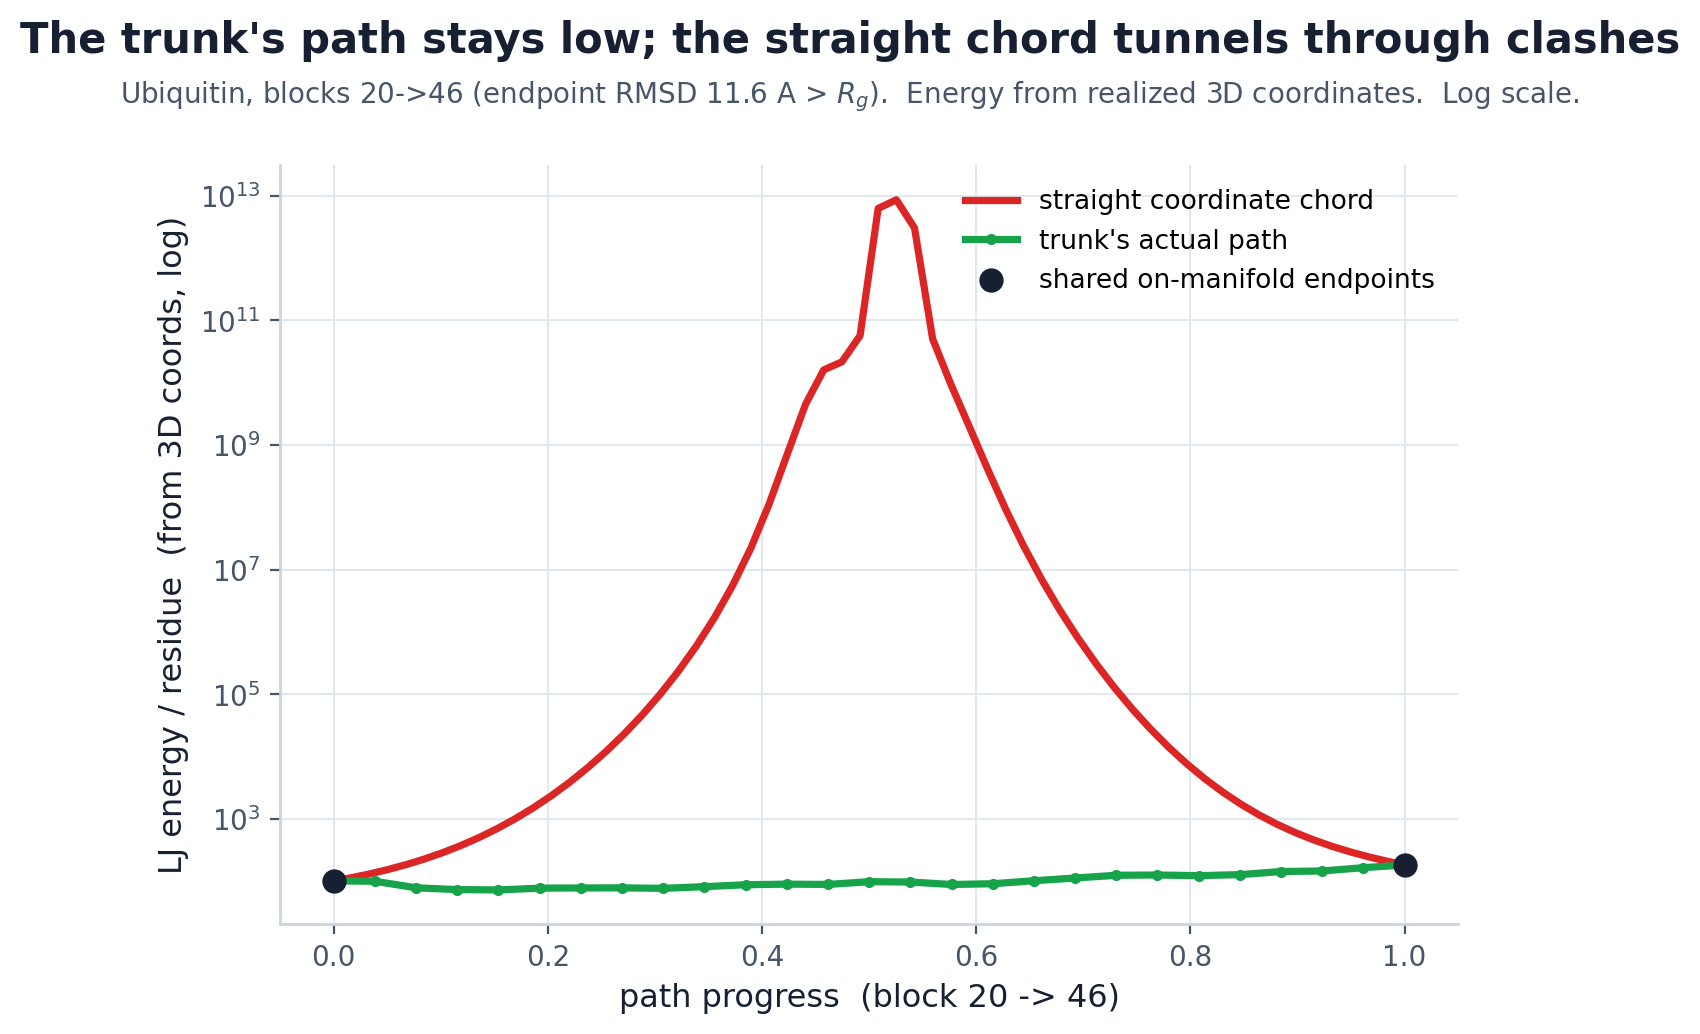
\includegraphics[width=0.95\linewidth]{figures/manifold_chord.png}
  \caption{Trunk path (green) vs.\ straight coordinate chord (red) between two
  on-manifold waypoints, energy from realized 3D coordinates. The chord tunnels
  through high-energy, sterically overlapping geometry; the trunk path stays low.
  \CHECK{regenerate as a clean ubq-only panel with log $y$-axis; the magnitude is
  a hard-LJ near-collision artifact, the honest claim is the qualitative
  separation.}}
  \label{fig:chord}
\end{figure}

\todofig{Four-distribution comparison of the potential-free headline metric
(minimum interatomic distance / steric-clash fraction): trunk-success,
trunk-failure, chord-success, chord-failure. The two trunk distributions overlap
and stay safe; both chord distributions hit atomic overlap. Generate by extending
\texttt{scripts/manifold\_chord\_experiment.py} to emit per-path min-distance and
clash-fraction over a success/failure protein set.}
{Trunk-path steric adherence is the same on failures as on successes; both chords
tunnel. The trunk navigates \emph{along} the realizable region rather than
through forbidden geometry.\label{fig:four-dist}}

\noindent Claim earned: the trunk navigates along the physically realizable region
rather than tunneling through forbidden geometry---not any path to the destination
works.

\subsection{It is not gradient descent; it is emergent}
\label{sec:not-gd}

Is the trunk descending energy by gradient steps? We measure
$\cos(\Delta z_t,\,-\nabla_z E)$.

\paragraph{The alignment is real but far below gradient descent.}
In $D\approx 7.4\times10^5$ dimensions \CHECK{$D=L^2\cdot128$; state $L$ used},
random directions are orthogonal to within $\pm 1/\sqrt{D}\approx 0.001$, so a
measured cosine of $\sim$0.05 is a $\sim$43$\sigma$ departure from chance
($p\sim10^{-401}$)---the energy-aligned component is real beyond any doubt
(random baseline $\sim$$10^{-4}$, Fig.~\ref{fig:cosine}). \CHECK{column meaning in
\texttt{cosine\_alignment\_summary.csv}: confirm the energy-gradient column and
the representative value; resolve the earlier $-0.01$ vs.\ $0.05$ discrepancy and
restate the GD-ruling-out argument consistently.}
But 0.05 is far below the $\approx 1.0$ that literal first-order gradient descent
would produce. Moreover, isotropic noise can only \emph{attenuate} a measured
cosine toward the orthogonal null, so 0.05 is a \emph{lower bound} on the true
alignment, not an estimate.\footnote{A clean direction diluted by per-coordinate
noise of magnitude $\sim$0.023 yields a measured cosine near 0.05; detectability
$\neq$ magnitude.}

\paragraph{Synthesis.}
The trunk does \emph{not} perform gradient descent on energy, yet its updates
carry a real, lower-bounded energy-aligned component, its path adheres to the
physically realizable region (\S\ref{sec:chord}), and it improves packing
favorability monotonically within that region
(\S\ref{sec:descent}--\S\ref{sec:false-protein}). It implements an amortized
procedure that \emph{arrives at} well-packed, sterically valid configurations
without \emph{descending toward} them by gradient steps.

\paragraph{Emergence (keystone).}
The trunk is trained on endpoints, not trajectories---it was never shown a folding
path. Both the steric path-adherence and the packing descent are therefore
properties of the learned procedure, not trained objectives. This closes the
deflationary readings that require energy to be present in the training signal.

\begin{figure}[t]\centering
  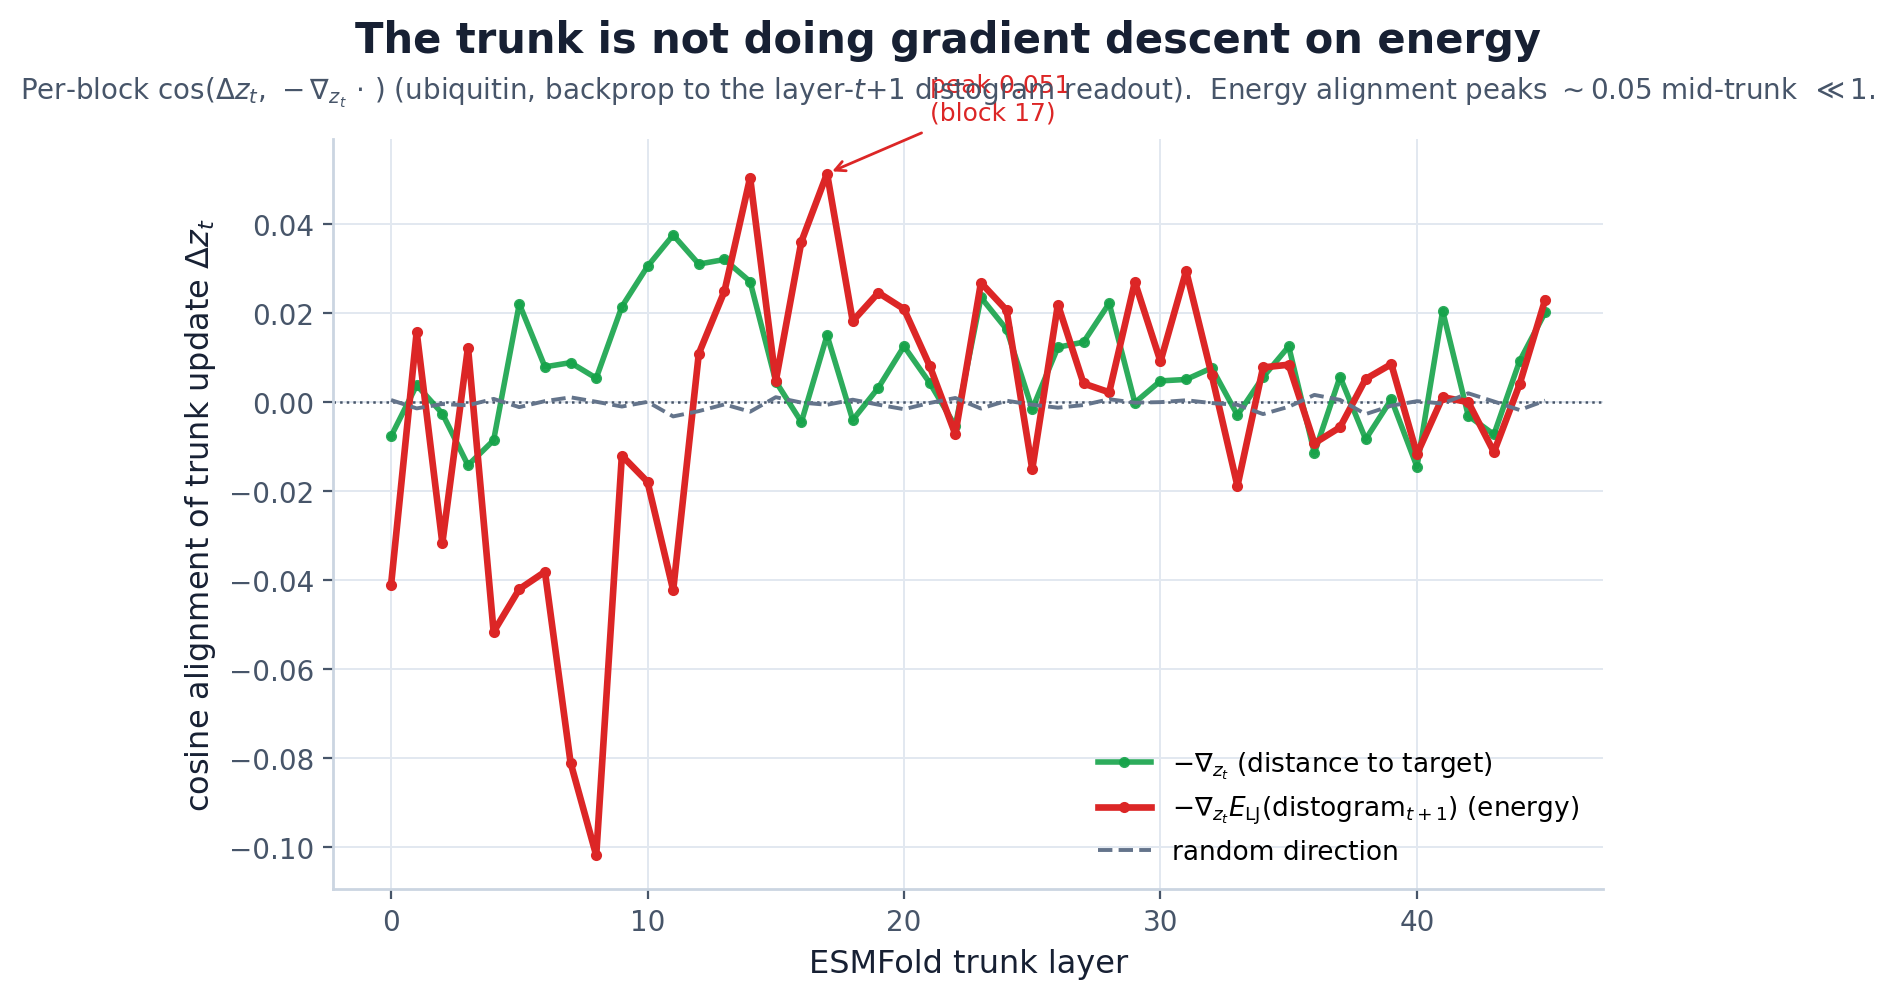
\includegraphics[width=0.8\linewidth]{figures/cosine_alignment.png}
  \caption{$\cos(\Delta z_t, -\nabla_z E)$ across layers and proteins. The
  alignment is small but vastly above the random-direction baseline
  ($\sim$$10^{-4}$) and far below the $\approx 1.0$ of literal gradient descent;
  with isotropic noise it is a lower bound on the true alignment.}
  \label{fig:cosine}
\end{figure}

% =====================================================================
\section{Limitations}
\label{sec:limitations}

\begin{itemize}[leftmargin=1.3em,itemsep=3pt]
\item \textbf{Energy claims are split and neither rests on a chosen potential.}
  The steric / path-adherence claim (\S\ref{sec:chord}) is geometric---excluded
  volume, reported as minimum interatomic distance---hence potential-free. The
  packing-descent claim (\S\ref{sec:descent}--\S\ref{sec:false-protein}) is
  established as attractive-regime by the magnitude argument (descent $\sim$5--10
  vs.\ clash scale $\geq 10^3$ under the \emph{same} potential), not by the LJ
  form. We deliberately do not claim potential-independence via a multi-potential
  sweep, since such potentials share a repulsive core and are not independent
  tests. Both claims concern coarse-grained C$\alpha$ geometry, not full-atom
  energetics.
\item \textbf{C$\alpha$-only geometry} via MDS embedding of probe distances; side
  chains, backbone torsions, and full clash terms are not captured.
\item \textbf{Faithfulness assumptions.} The readout rests on the
  gradual-geometric-change assumption (imported, supported by \citet{lu2026phase},
  not proven here) and on the anchor being in-distribution at the final layer.
\item \textbf{Scope of content.} The probe reads geometric content specifically;
  non-geometric content in $z$ is outside the method's scope.
  \NEXTPAPER{the trunk carries information beyond the geometric content the probe
  reads; characterizing it is a direction we are pursuing.}
\item \textbf{Mechanism characterized negatively.} We show not-first-order-GD and
  emergent; the positive identity of the amortized procedure is not established.
\item \textbf{Scale / generality.} $N=$\CHECK{number of proteins} proteins,
  ESMFold specifically; generality beyond ESMFold is unverified here.
\end{itemize}

% =====================================================================
\section{Future work}
\label{sec:future}

\begin{itemize}[leftmargin=1.3em,itemsep=3pt]
\item \textbf{Identify the amortized procedure} positively (proximal step?
  preconditioned / natural gradient? alternating projection?), following directly
  from the negative characterization in \S\ref{sec:not-gd}.
\item \textbf{Causal intervention via the faithful probe:} the repair
  experiment---inject a high-energy perturbation and test whether the trunk
  restores manifold adherence---the interventional version of \S\ref{sec:chord}'s
  observational result.
\item \textbf{Non-geometric content} the probe does not capture, and its role in
  the computation.
  \NEXTPAPER{stake priority only; do not reveal the reliability metric.}
\end{itemize}

% =====================================================================
\section{Conclusion}
\label{sec:conclusion}

We presented a faithful per-layer geometric readout of the ESMFold trunk---content
via reconstruction of $z_t$, not decodability via supervision; anchored
in-distribution at the final layer, with no native structure in the loss---and
used it to show that the trunk's intermediate beliefs adhere to the low-energy
manifold even when the model folds incorrectly. The adherence is emergent from
endpoint-only training and is not gradient descent: the trunk implements an
amortized procedure that arrives at well-packed, sterically valid configurations
without descending toward them by gradient steps, while a straight path between
the same waypoints tunnels through forbidden geometry. This is a reading of what
the trunk \emph{believes}, not merely what is decodable from it, and it supports a
mechanistic account of single-pass folding as manifold-adherent reorganization.

% =====================================================================
\begin{thebibliography}{9}
\small
\bibitem[Adams et al.]{adams_sae} Adams et al. \emph{Sparse autoencoders for
protein language models.} \VERIFY{full citation + claim.}
\bibitem[AlphaInterp]{alphainterp} AlphaInterp: interpretability for AlphaFold~3.
\VERIFY{authors, venue, claim.}
\bibitem[Jumper et al.~2021]{alphafold2} Jumper et al. \emph{Highly accurate
protein structure prediction with AlphaFold.} Nature, 2021. \VERIFY{per-block
structure-module supervision, Supp.\ Methods 1.14.}
\bibitem[Lin et al.~2023]{esmfold} Lin et al. \emph{Evolutionary-scale prediction
of atomic-level protein structure with a language model (ESMFold).} Science, 2023.
\bibitem[Lu et al.~2026]{lu2026phase} Lu et al. \emph{Phase diagram of distance
decodability across depth.} 2026. \VERIFY{linear decodability + gradual
accumulation attribution.}
\bibitem[Reticular]{reticular_msae} Reticular. \emph{Matryoshka sparse
autoencoders on ESM2-3B.} \VERIFY{citation + claim.}
\bibitem[Simon \& Zou]{simon_interplm} Simon \& Zou. \emph{InterPLM:
interpreting protein language models with sparse autoencoders.} \VERIFY{citation
+ claim.}
\end{thebibliography}

\end{document}
